\documentclass[titlepage,11pt]{article}

\textwidth 6.5in
\textheight 9in
\oddsidemargin -0.2in
\topmargin -0.5in

\usepackage{indentfirst,graphics,alltt,epsfig,color}

\title{iBioSim Version 2.5 \\ Tutorial}

\author{Chris J. Myers}

\begin{document}

\maketitle

%show only subsection granularity in the toc
%\setcounter{tocdepth}{2} 
  
\tableofcontents

\clearpage

\section{Introduction}

\noindent
{\tt iBioSim} has been developed for the modeling, analysis, and design of genetic circuits.  While {\tt iBioSim} primarily targets models of genetic circuits, models representing metabolic networks, cell-signaling pathways, and other biological and chemical systems can also be analyzed.  {\tt iBioSim} includes the following components: 

\begin{itemize}
\item Model Editor - a tool to create a model of a genetic circuit or other biological system.
%\item SBOL Browser - a tool to view SBOL files and associate DNA components to model elements.
\item Analysis Tool - an abstraction-based ODE, Monte Carlo, and Markov analysis tool.
\item Learn Tool - a tool to learn a model from \emph{time series data} (TSD).
\item TSD Graph Editor- a tool to visualize TSD files. 
\item Histogram Graph Editor - a tool to visualize probability data. 
\end{itemize}

This tutorial illustrates each of these features of {\tt iBioSim} using a simple model for the \emph{cI} and \emph{cII} genes and the $P_R$ and $P_{RE}$ promoters from the phage $\lambda$ decision circuit.  

% TODO: add figures and more description of the example

\section{Project Management}

\noindent
Within {\tt iBioSim}, all files are collected within projects.   A project is a collection of models, analysis views, learn views, and graphs.  As shown below, {\tt iBioSim} displays all project files on the left, the open models, views, and graphs on the right, and a log of all external commands on the bottom.  The menu bar is located on the top of the window in the Windows and Linux versions.  It is located on the top of the screen in the MacOS version.

\begin{center}

\includegraphics[width=160mm]{screenshots/iBioSim}
\end{center}

\noindent
To create a new project, select New $\rightarrow$ Project from the File menu as shown below.  You will then be prompted to browse to a desired location and to give a name to the project directory.  Enter the name {\tt Tutorial}.  After you do this, click the new button and a new project directory will be created.  

\begin{center}
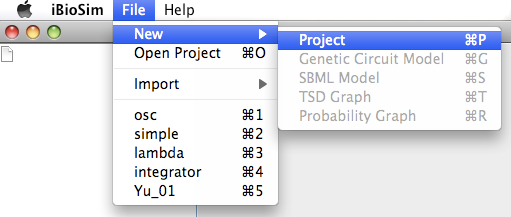
\includegraphics[width=60mm]{screenshots/project}
\end{center}

\section{Model Editor}

\noindent
After you have created a project, you can create a new model to add to the project by selecting New $\rightarrow$ Model from the File menu as shown below. You will then be prompted to enter a model ID.  Enter {\tt lambda}.  At this point, a Model editor will open in a new tab.

\begin{center}
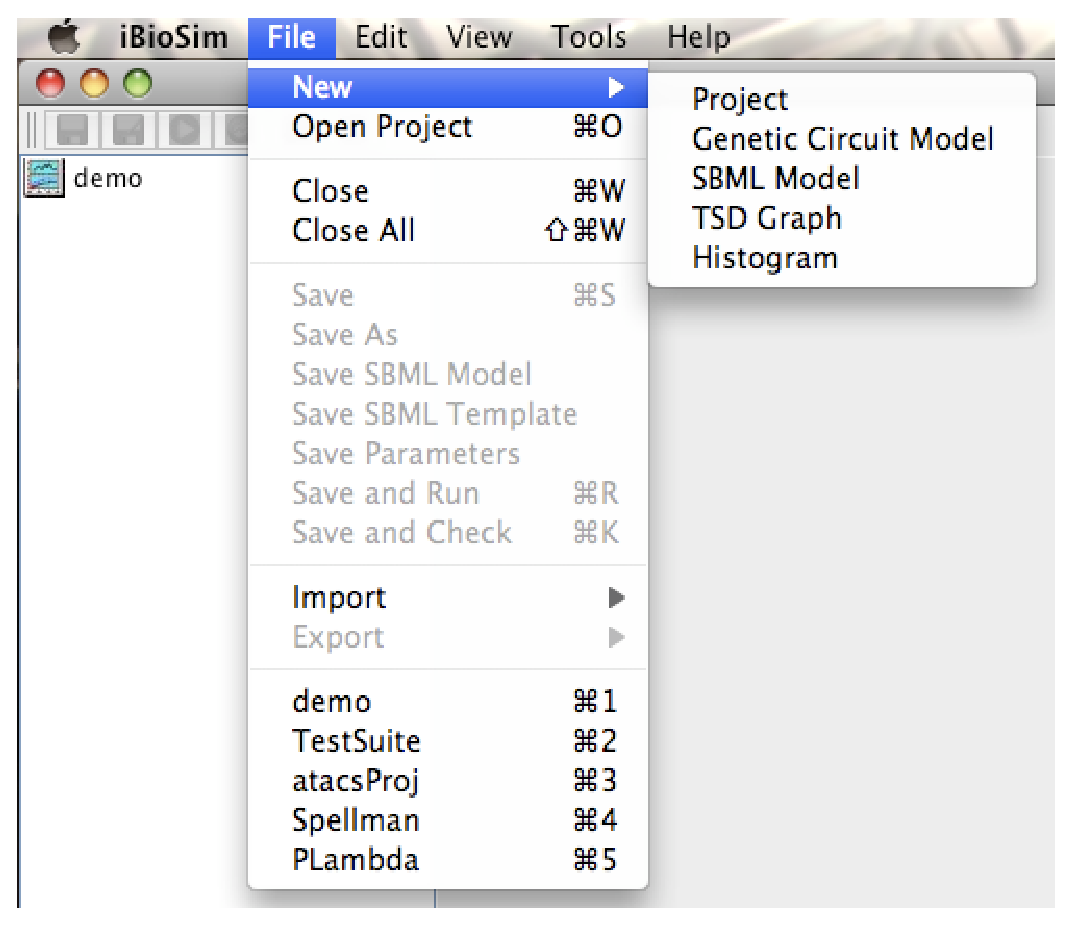
\includegraphics[width=80mm]{screenshots/newModel}
\end{center}

\begin{center}
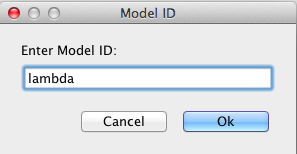
\includegraphics[height=25mm]{screenshots/ModelId}
\end{center}

\begin{center}
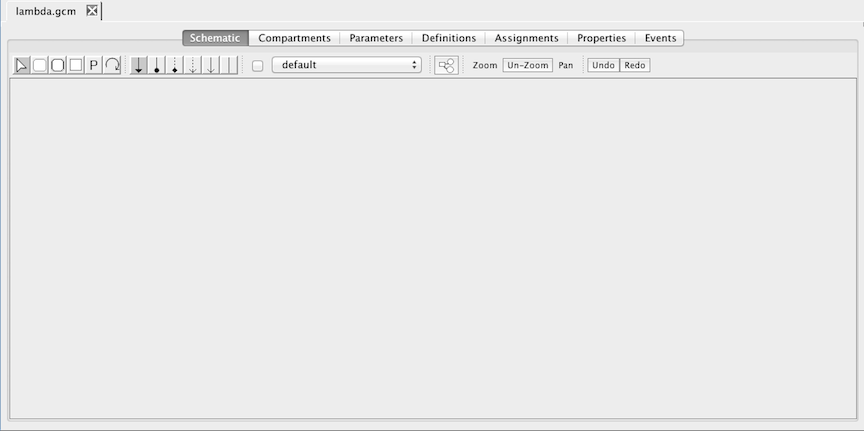
\includegraphics[width=160mm]{screenshots/ModelEditor}
\end{center}

Compartments are the membrane-enclosed regions where species can be found and reactions take place.  {\tt iBioSim} creates a default compartment initially with the ID of Cell.  If you click on the schematic within the Cell compartment, it brings up the compartment editor.  Uncheck the ``Is Mapped to a Port''.  This indicates that this compartment should be enclosing this model and not replaced when instantiated in a larger model.  Once you press OK, you will notice that the compartment now has rounded corners to indicate that this is membrane enclosed by the compartment Cell.

\begin{center}
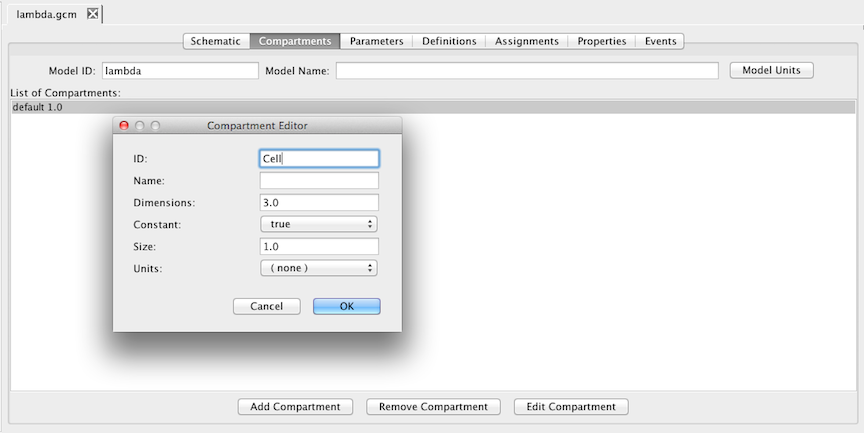
\includegraphics[width=160mm]{screenshots/compartment}
\end{center}

To add a chemical species, select the Add Species icon 
\includegraphics{../gui/icons/modelview/add_species_selected} and click on the schematic canvas.  This will drop a new species with default ID and other values.  You may change these defaults by clicking on the selection icon 

\includegraphics{../gui/icons/modelview/select_mode_selected}, and
double-clicking on the species to open the Species Editor.  In this case, let us change the ID to CI, and click on degrades checkbox.  We will leave all other values at their default values.  One thing that is important to note is that when this model is analyzed a default degradation reaction will be created which has a rate of 0.0075.  

\begin{center}
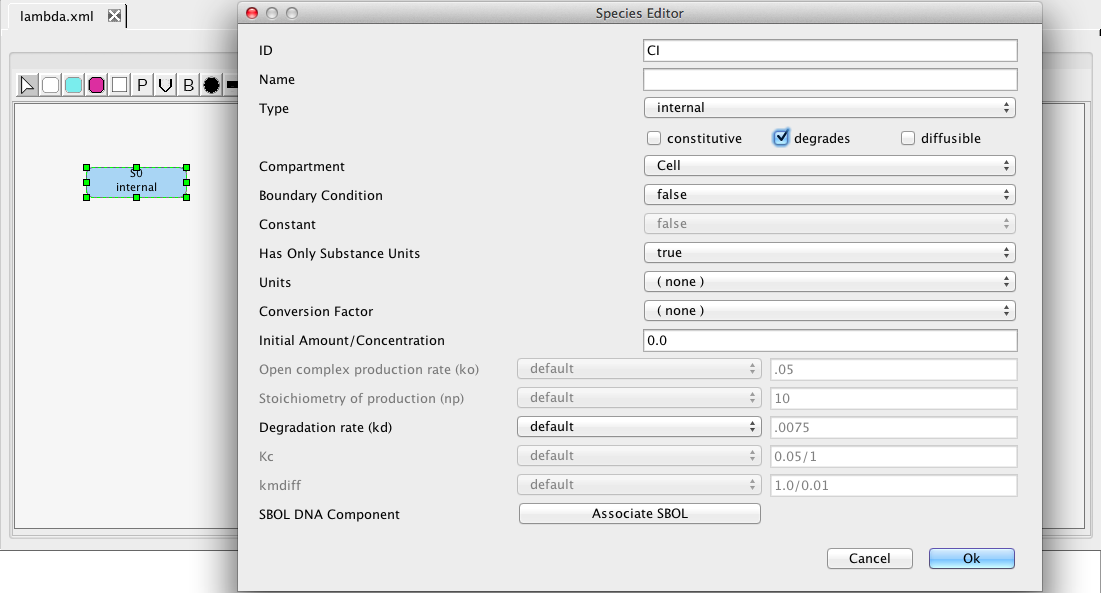
\includegraphics[width=160mm]{screenshots/species}
\end{center}

Add another species for the CI dimer molecule.  The next step is to add a complex-formation reaction to convert CI monomers into CI dimers.  Select the complex formation icon 
\includegraphics{../gui/icons/modelview/bio_activation_selected}, highlight the CI species, and, while holding the mouse button, stretch the complex formation arc to the S1 species.  Next, edit this species to set its ID to CI2 and select that it degrades.  This species is created using a complex-formation reaction with an equilibrium constant of 0.1.  Change default to custom for the complex formation equilibrium and set it to this value as shown below.

\begin{center}
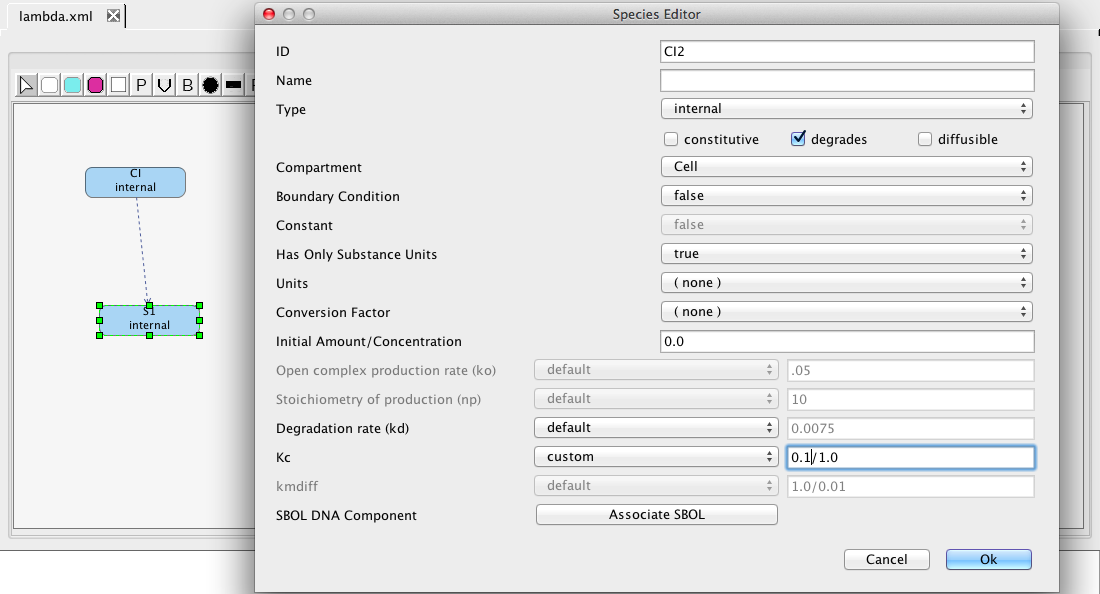
\includegraphics[width=160mm]{screenshots/species2} 
\end{center}

If you double-click on the complex formation arc, an influence editor will open which indicates that this is a complex formation arc and the stoichiometry of binding (i.e., the number of molecules of the source species used to construct the sink species) is 2.  The default in this case is correct as it does take two molecules of CI to make CI2.

\begin{center}
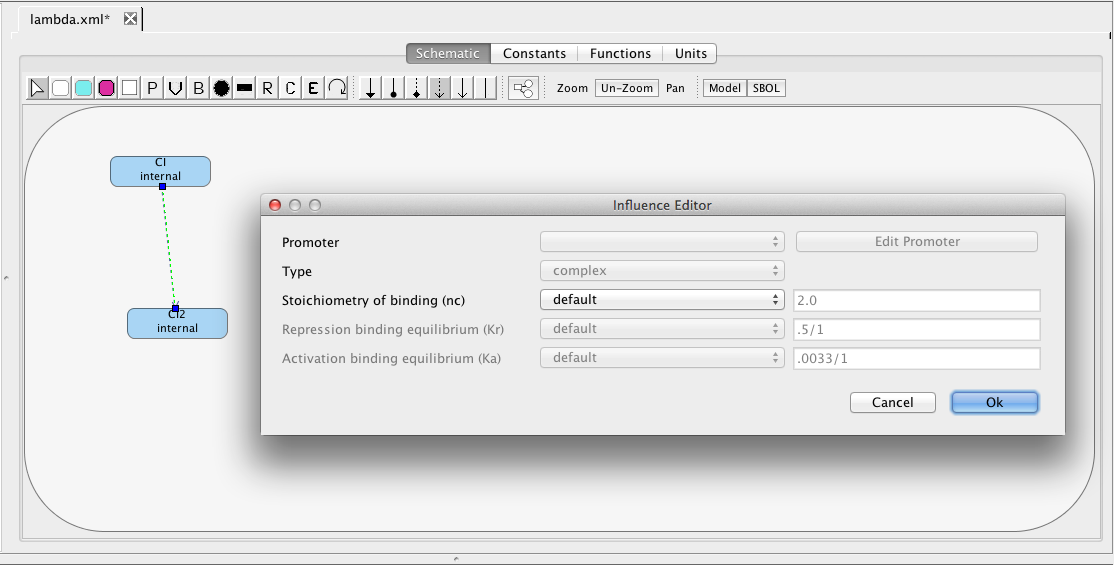
\includegraphics[width=160mm]{screenshots/complex} 
\end{center}

Next, let's add the PR promoter, which initiates transcription of the gene that produces the protein CII.  To do this, select the promoter icon 
\includegraphics{../gui/icons/modelview/promoter_mode_selected} and click on the schematic canvas to drop the promoter with a default ID and parameter values.  Double-click on the promoter to bring up the promoter editor.  Change the ID to PR, customize the RNAP binding equilibrium to be 0.69422, and set the open complex production rate to be 0.014. 
 
\begin{center}
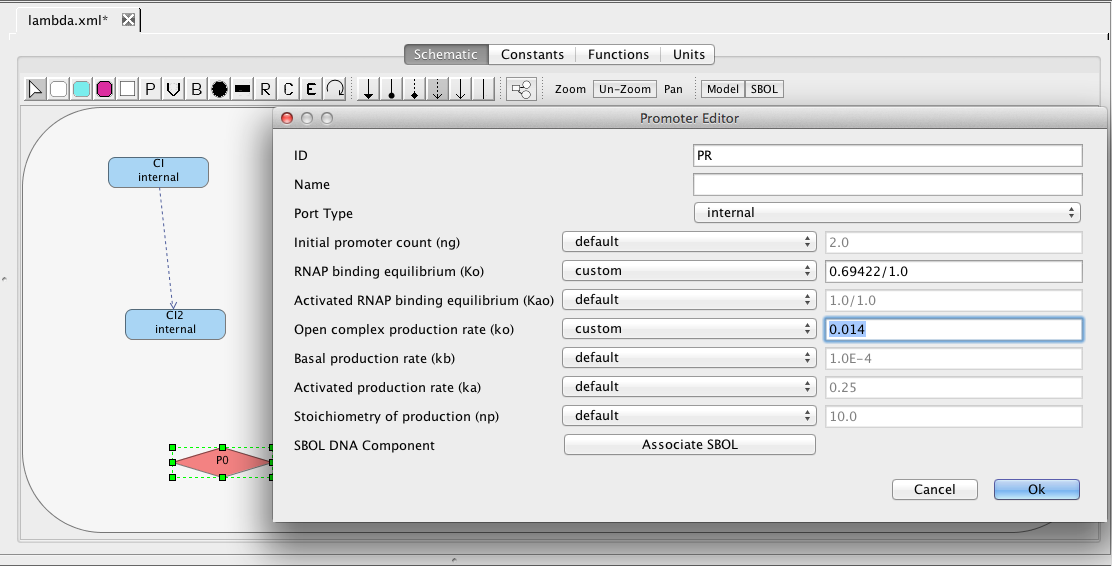
\includegraphics[width=160mm]{screenshots/promoter} 
\end{center}

The PR promoter is repressed by the CI2 species.  To create this relationship, select the repression arc icon 

\includegraphics{../gui/icons/modelview/inhibition_selected}, highlight the CI2 species, and, while holding the mouse button, stretch the repression arc to the PR promoter.  Next, double-click on the repression arc to bring up the influence editor.  In this editor, customize the stoichiometry of binding to 1, indicating that just one CI dimer is necessary to repress this promoter, and change the repression binding equilibrium to 0.2165.

\begin{center}
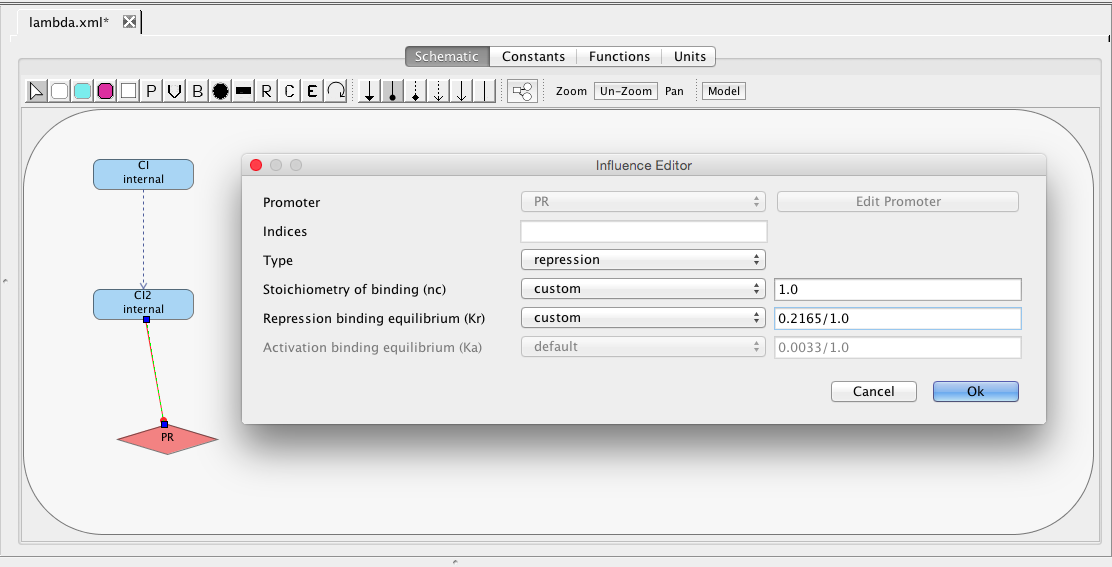
\includegraphics[width=160mm]{screenshots/repression} 
\end{center}

As mentioned earlier, the PR promoter initiates the production of the CII species.  Add the CII species following the steps given earlier for adding a species (be sure to mark that it degrades).  Then, highlight the PR promoter and, while holding the mouse button, stretch the production arc to the CII species.  Note that the icons selected for this are not important because all arcs from promoters to species are always production arcs.

\begin{center}
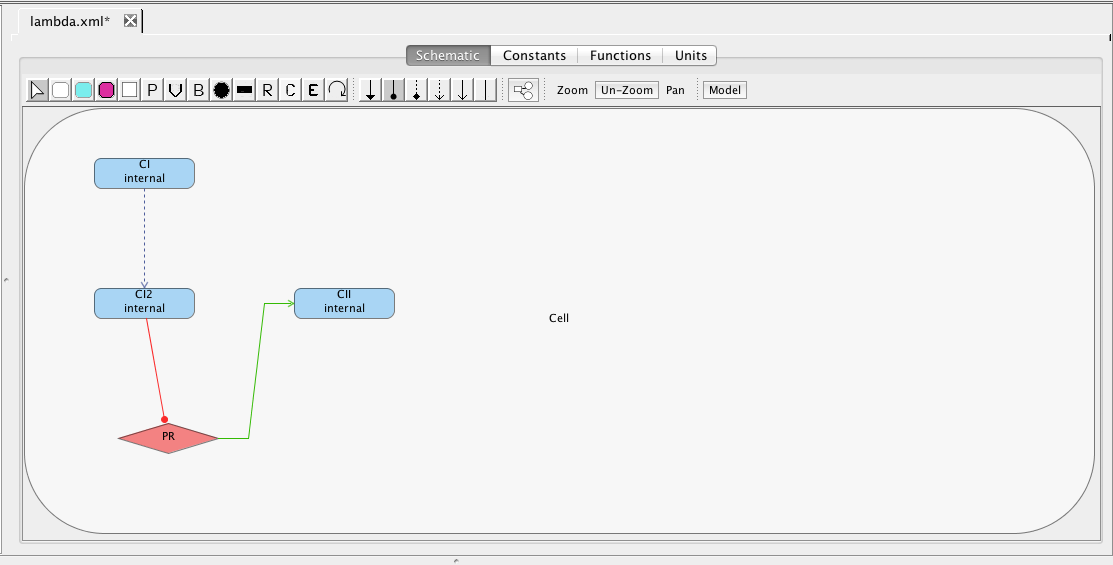
\includegraphics[width=160mm]{screenshots/production}
\end{center}

Finally, CII species activates the production of the CI species from the PRE promoter.  Promoters do not need to always be drawn.  They can also be implicit on an influence.  To add an activation arc with an implicit promoter, select the activation arc icon 
\includegraphics{../gui/icons/modelview/activation_selected}, highlight the CII species, and, while holding the mouse button, stretch the activation arc to the CI species.  This creates not only the influence but also a default promoter.  Double-click on the activation arc to bring up the influence editor.  In this editor, customize the stoichiometry of binding to 1, indicating that just one CII molecule is necessary to activate this promoter, and change the activation binding equilibrium to 0.00161.  Finally, click on the Edit Promoter button and change the ID of this promoter to PRE.  Also, customize the RNAP binding equilibrium to be 0.01, the basal production rate to be 0.00004, and the activated production rate to be 0.015.

\begin{center}
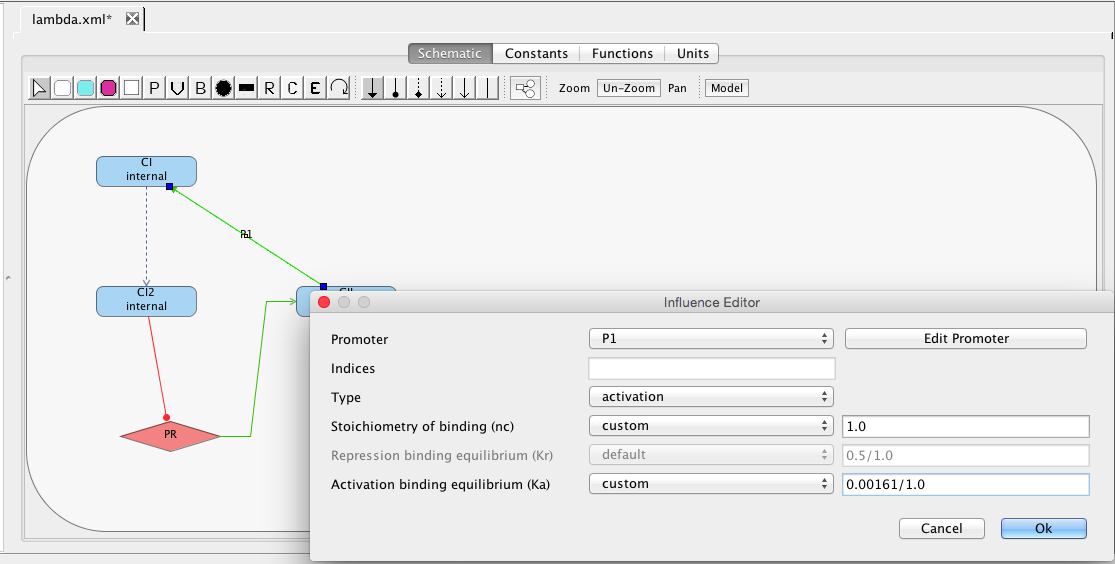
\includegraphics[width=160mm]{screenshots/activation}
\end{center}

\begin{center}
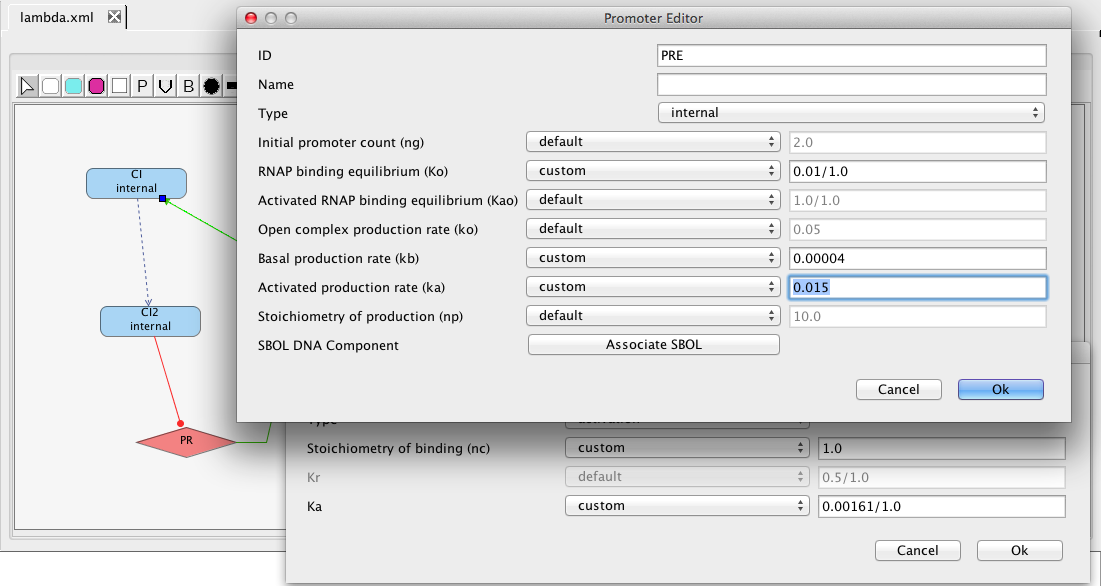
\includegraphics[width=160mm]{screenshots/activated_promoter}
\end{center}

Next, let's go look at some of the other model tabs.  Click on the Functions tab.  Here one can add/remove/edit definitions for functions.  Click on Add Function, and let's create a function to compute the total number of molecules where $x$ is the number of monomers and $y$ is the number of dimers.  Let's give this function an ID of total with arguments $x$ and $y$, and a definition of $x + 2 * y$.

\begin{center}
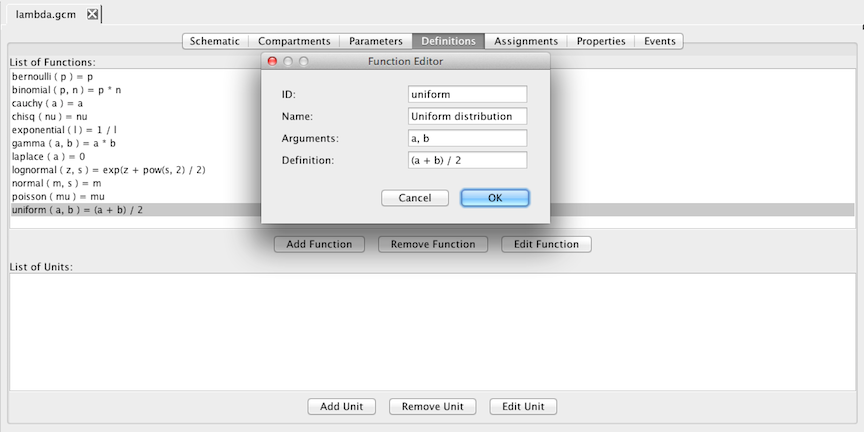
\includegraphics[width=160mm]{screenshots/function}
\end{center}

Click on the Units tab.  Unit definitions allow the user to create custom units for use in models.  As an example, click Add Unit and enter the ID nanoMole.  A unit is defined using pre-defined base units.  Click on Add to List and find mole in the Kind combo box, and change the scale to $-9$ to define a nanoMole in terms of moles. The exponent and multiplier are real numbers, and the scale is an integer that specifies the relationship between the derived unit and the base unit using the relation below:
\begin{eqnarray*}
\mathrm{unit} & = & (\mathrm{multiplier} * 10^\mathrm{scale} * \mathrm{baseUnit})^\mathrm{exponent}
\end{eqnarray*}
Follow the same steps to create a unit for microLitre.

\begin{center}
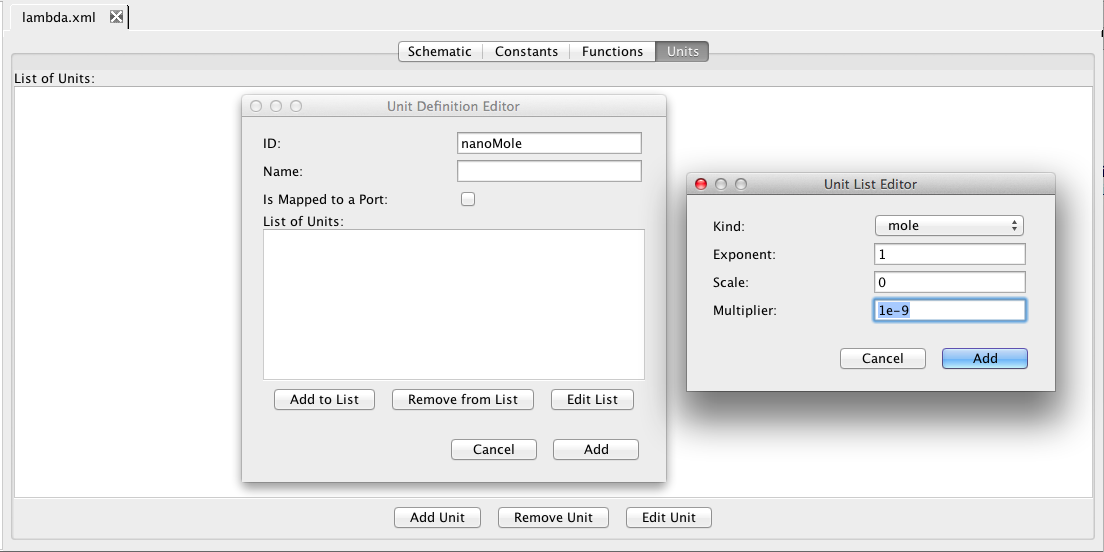
\includegraphics[width=160mm]{screenshots/units}
\end{center}

Next, click on the Schematic tab.  Then, click on the Model button to bring up a window of default units for this model.  These are the units to be used for various things when no units are provided.  For this model, let's make the Substance Units be in nanoMoles, Time Units be in seconds, and Volume Units be in microLitres.  The Extent Units indicate the units of change for reactions.  Let's make that also be nanoMoles.

\begin{center}
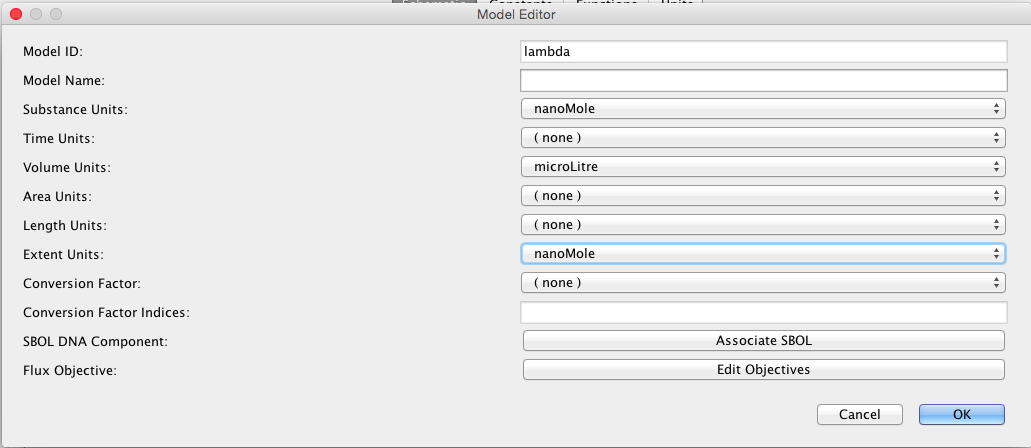
\includegraphics[width=160mm]{screenshots/ModelUnits}
\end{center}

Next, click on the Constants tab.  This tab includes the default model generation parameters as well as additional global variables.  The model generation parameters are used for default values when creating a reaction-based model from our higher level model.  These parameters can be edited by selecting them and entering a new initial value.  They should not be removed.  Note that new global constants can also be added by the user, if desired.

\begin{center}
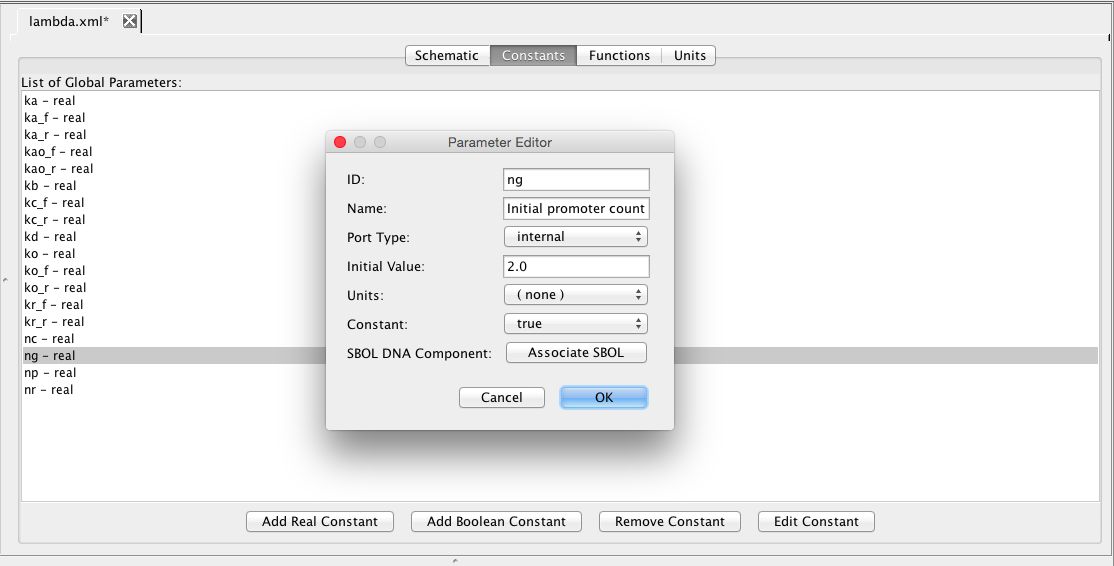
\includegraphics[width=160mm]{screenshots/GCMparam}
\end{center}

While you can add a global variable here, the preferred way is to add it on the schematic.  Click on the Schematic tab.  Select the add variable icon 
\includegraphics{../gui/icons/modelview/variable_mode_selected}, and click a location to add the variable to the schematic.  Then, click on the selection icon 

\includegraphics{../gui/icons/modelview/select_mode_selected}, and double click on the variable to open the Parameter Editor.  Change the ID to CI\_total, for the total amount of the species CI in both monomer and dimer form.  Its units are in nanoMole and it is not constant.  

\begin{center}
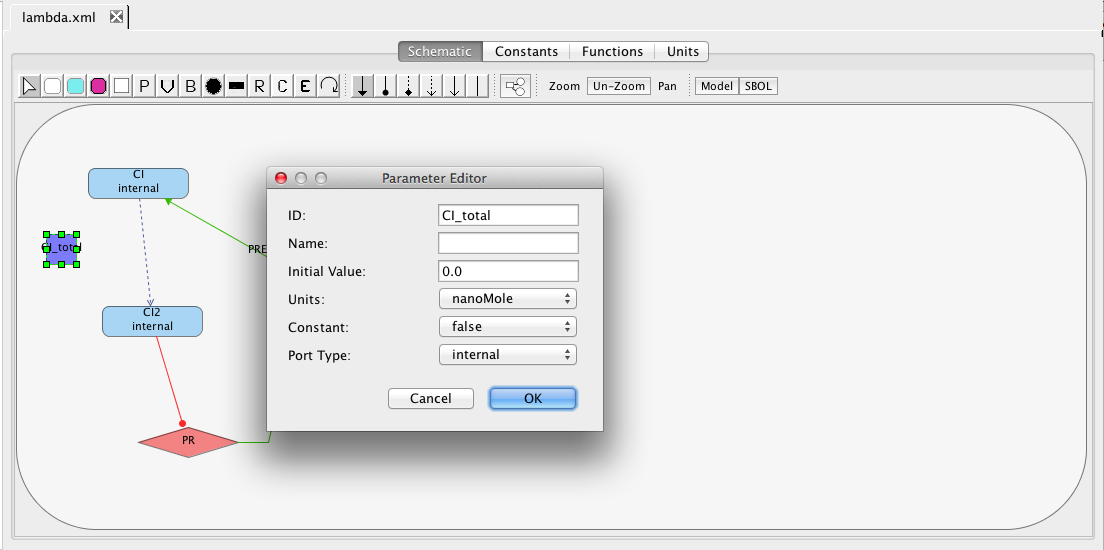
\includegraphics[width=160mm]{screenshots/parameter}
\end{center}

% Now, let's go to the Assignments tab.  This tab includes initial assignments and rules.  Initial assignments are used when you want the initial value of a compartment size, species amount or concentration, or parameter to be determined by a mathematical equation rather than a constant.  Click on Add Initial, select CI2 as the Symbol, and enter the assignment 5*CI, which causes CI2's initial value to be five times that of CI's initial value.  Therefore, if we were to go change CI's initial value, CI2's initial value would also change due to this initial assignment.

% \begin{center}
% 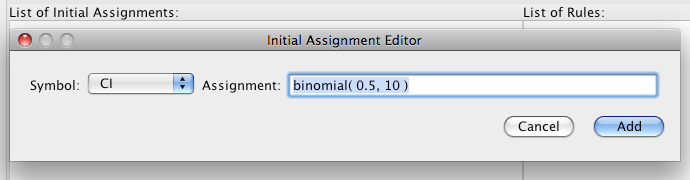
\includegraphics[width=160mm]{screenshots/initial}
% \end{center}

Now, let's create a rule to compute the value of CI\_total.  There are three types of rules: algebraic, assignment, and rate.  Algebraic rules are used to specify relationships that must be maintained.  Assignment rules are used to define one variable in terms of a mathematical expression.  Finally, rate rules are used to indicate a differential equation to govern the evolution of a variable in terms of a mathematical expression on other variables.  To add a rule, select the add rule icon

\includegraphics{../gui/icons/modelview/rule_mode_selected}.  In the Rule editor, 
select Assignment, select the variable CI\_total, and enter the expression total(CI,CI2).  This uses our new function to compute that the amount of CI in total is the number of monomer molecules plus two times the number of dimer molecules.

\begin{center}
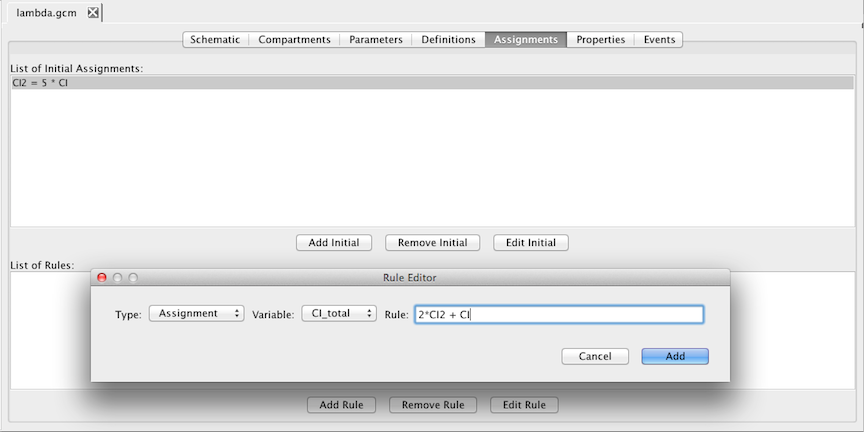
\includegraphics[width=160mm]{screenshots/rule}
\end{center}

% The next tab is the properties tab.  Here you can specify probabilistic temporal logic properties using \emph{Continuous Stochastic Logic} (CSL) that you wish to check.  For example, the property shown,
% Pr\{PF[0,2100](CI>20\}, would ask the analyzer to determine the probability that CI exceeds 20 molecules within 2100 seconds.

% \begin{center}
% 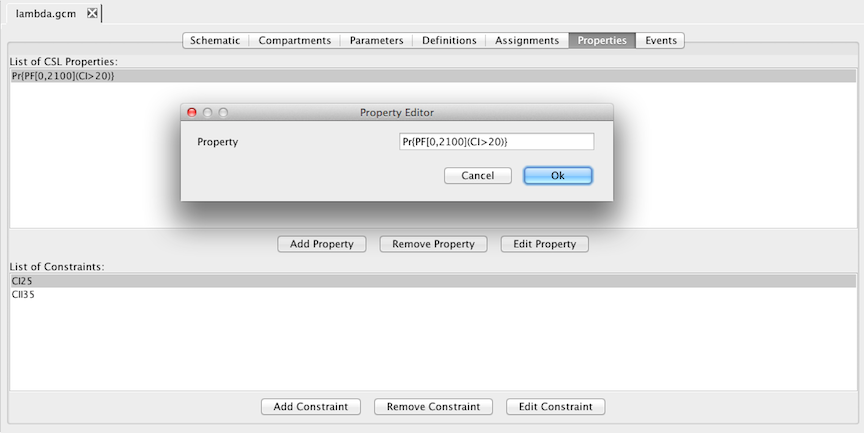
\includegraphics[width=160mm]{screenshots/properties}
% \end{center}

Next, let's add a constraint.  A constraint is a condition that must be satisfied or simulation should terminate.  To add a constraint, select the add constraint icon

\includegraphics{../gui/icons/modelview/constraint_mode_selected}.  Add a constraint that states that CI remains less than or equal to 20 molecules as shown below.  Add a second constraint that states that CII remains less than or equal to 50 molecules.

\begin{center}
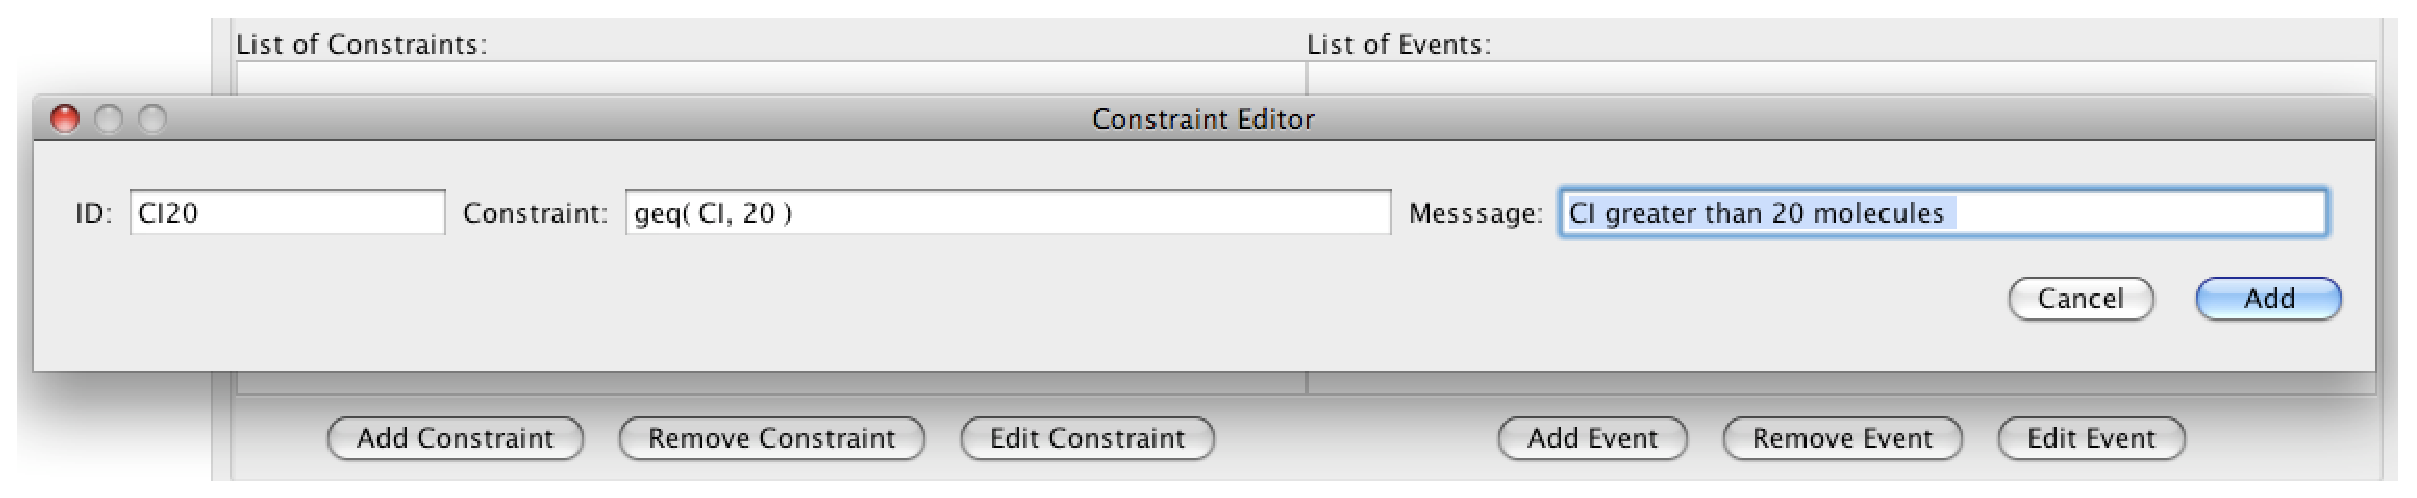
\includegraphics[width=160mm]{screenshots/constraint}
\end{center}

Finally, let's add an event.  Events are used to specify discrete state changes.  For example, let's describe an event for cell division.  Click on the Add Event button, enter the ID CellDivision, trigger true, and delay of 2100.  The trigger specifies the condition that should be satisfied to enable this event.  In this case, we want it to be enabled initially.  The delay indicates the time after which it is enabled that it should execute.  Finally, select the Dynamic Process of Symmetric Division.  This combination results in a cell division event at 2100 seconds after simulation begins.  The event assignments specify the state change(s) for this event.  Click on the Add Assignment button and select the CI variable, and enter the assignment CI / uniform(1,2).  In other words, the number of molecules is being divided between the two daughter cells with a random distribution.  Similarly, add event assignments to divide up CI2 and CII.

\begin{center}
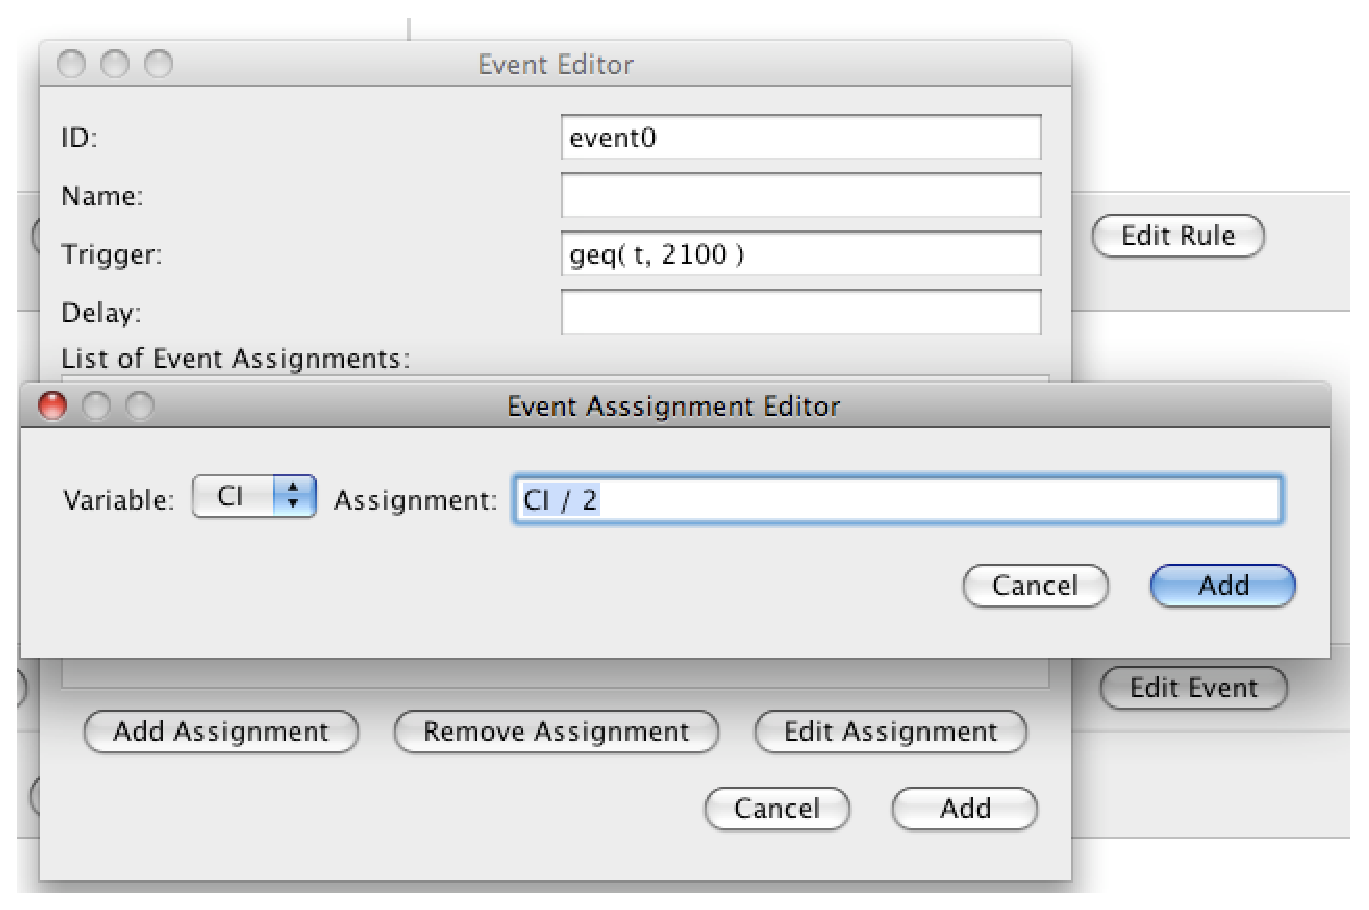
\includegraphics[width=160mm]{screenshots/event}
\end{center}

At this point, you should have a model that looks like the one below (though locations of elements may be different).  Now, let's make sure the model is saved by either clicking on the Save icon 
\includegraphics{../gui/icons/save} or selecting the Save option from the File menu.

\begin{center}

\includegraphics[width=160mm]{screenshots/save}
\end{center}

\section{Analysis Tool}

This section describes how to analyze the model just created.  The first step is to create an analysis view.  To do this, right-click on the model file and select Create Analysis View.  Enter the analysis ID {\tt lambda} or just press enter.  At this point, a new analysis view should open.  You should also notice that an icon appears next to your model file.  When you click on this, it will show you all of the analysis and learn views associated with this model.

\begin{center}
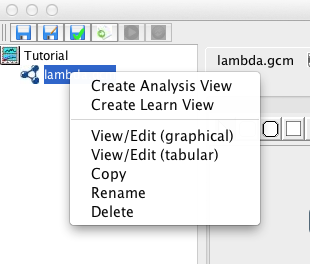
\includegraphics[height=60mm]{screenshots/GCMAnalysis}\\
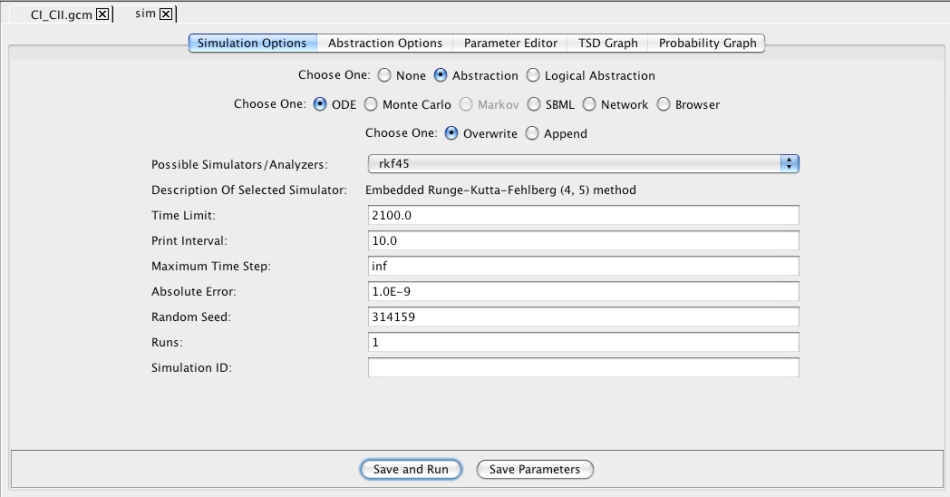
\includegraphics[width=160mm]{screenshots/analysisView}
\end{center}

In order to perform analysis, the analysis tool first converts the model into a reaction-based model in the \emph{Systems Biology Markup Language} (SBML).  There are three different ways to see the reaction-based model that is produced.  If GraphViz is installed on your computer, you can select Network for your Simulation Type.  Then, either press the Save and Run icon 
\includegraphics{../gui/icons/run-icon} or select the Save and Run option from the File menu.  The result will be a GraphViz window that will open to show the reaction-based model such as the one shown below for our example.  If it does not open in GraphViz, make sure that you have files with the {\tt .dot} file extension associated with GraphViz on your computer.  You can also view the model in a web browser by selecting Browser for your simulation type.  In this case, you should ensure that you have files with the {\tt .xhtml} extension associated with your favorite browser.  Finally, you can save the reaction-based model by selecting Model as your simulation type.  In this case, you must provide a new model ID.  This new model will appear in your project and it can be opened in the Model Editor.  Since this model does not include any layout information, you will need to either lay it out by hand or using one of the default layout routines selectable using the Apply Layout icon    
\includegraphics{../gui/icons/modelview/choose_layout_selected},

\begin{center}
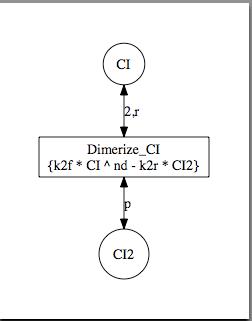
\includegraphics[width=120mm]{screenshots/viewNetwork}
\end{center}

\begin{center}
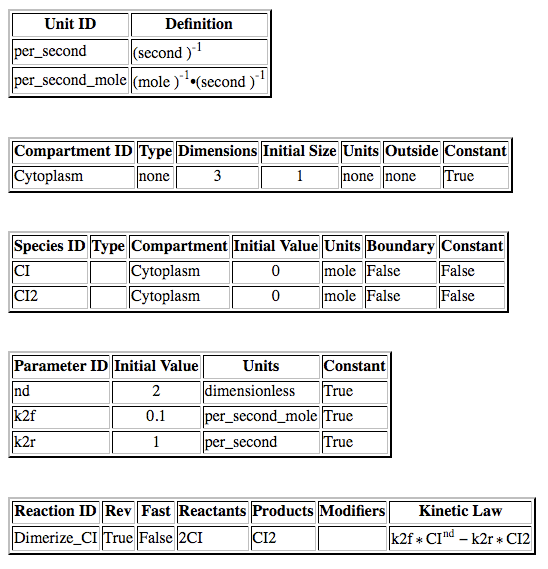
\includegraphics[width=160mm]{screenshots/viewBrowser}
\end{center}

\begin{center}
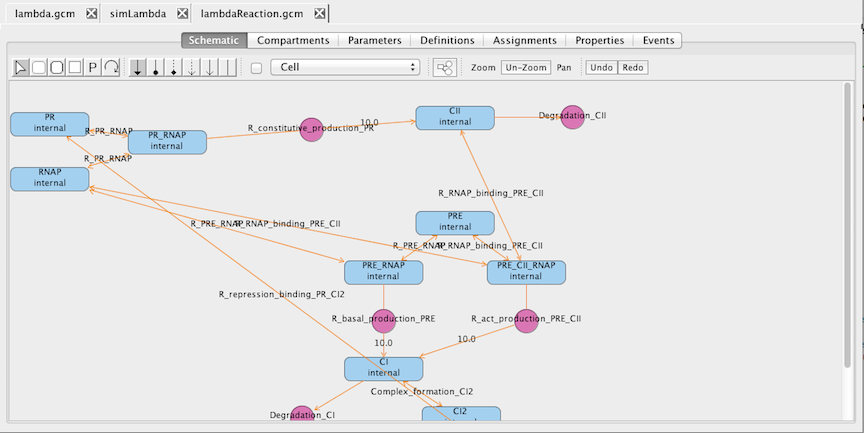
\includegraphics[width=160mm]{screenshots/reactionModel}
\end{center}

Next, click on the SBML elements tab.  This tab allows you to select which SBML model elements to include in your analysis.  This includes initial assignments, rules, constraints, and events.  Initially, let's only include the rule to compute CI\_total.  Uncheck all the other elements.

\begin{center}
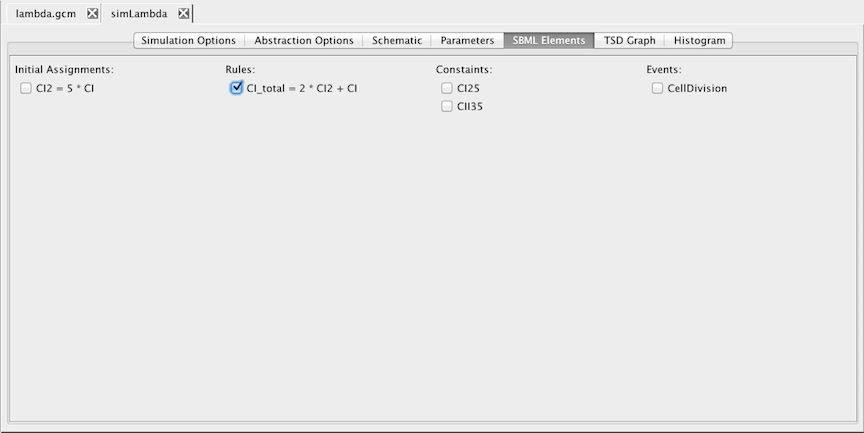
\includegraphics[width=160mm]{screenshots/SBMLElements}
\end{center}

Now, go back to the simulation options tab.  Here, change the simulation type back to ODE, change the time limit to 2100.0, change the print interval to 10.0, and enter a Simulation ID of {\tt ode}.  Then, either press the Save and Run icon 
\includegraphics{../gui/icons/run-icon} or select the Save and Run option from the File menu.
After the simulation completes, click on the TSD Graph tab.  Double-click on the graph to bring up the graph editor.
Open the {\tt ode} simulation, highlight Average, select CI\_total and CII, change the Title to ``ODE Simulation Results'', change the X-Axis Label to ``Time (seconds)'', and change the Y-Axis Label to ``Number of Molecules''.  
Press the OK button.  

\begin{center}
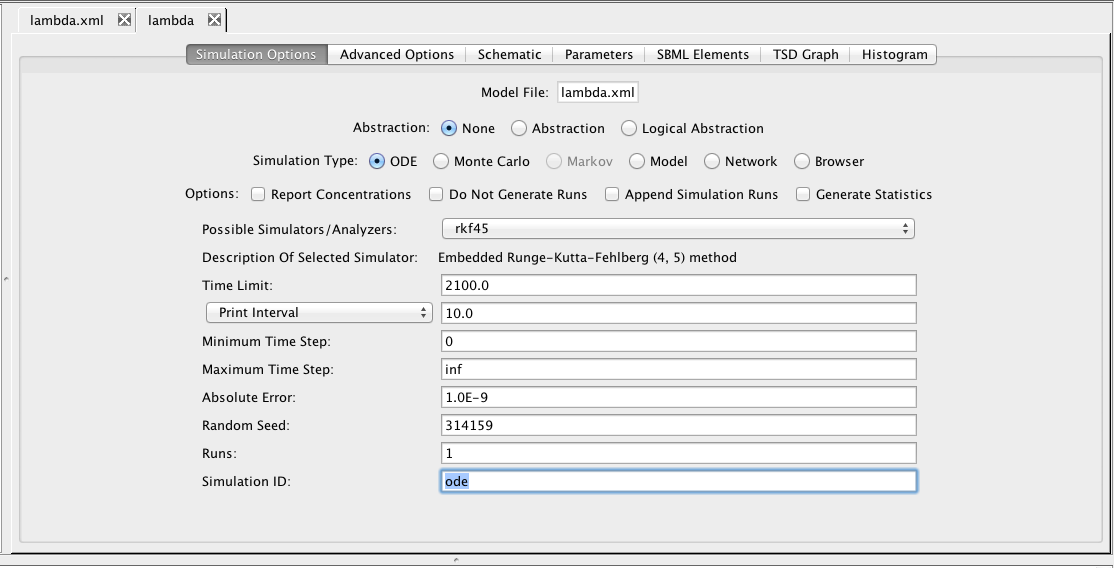
\includegraphics[width=160mm]{screenshots/odeSim}\\
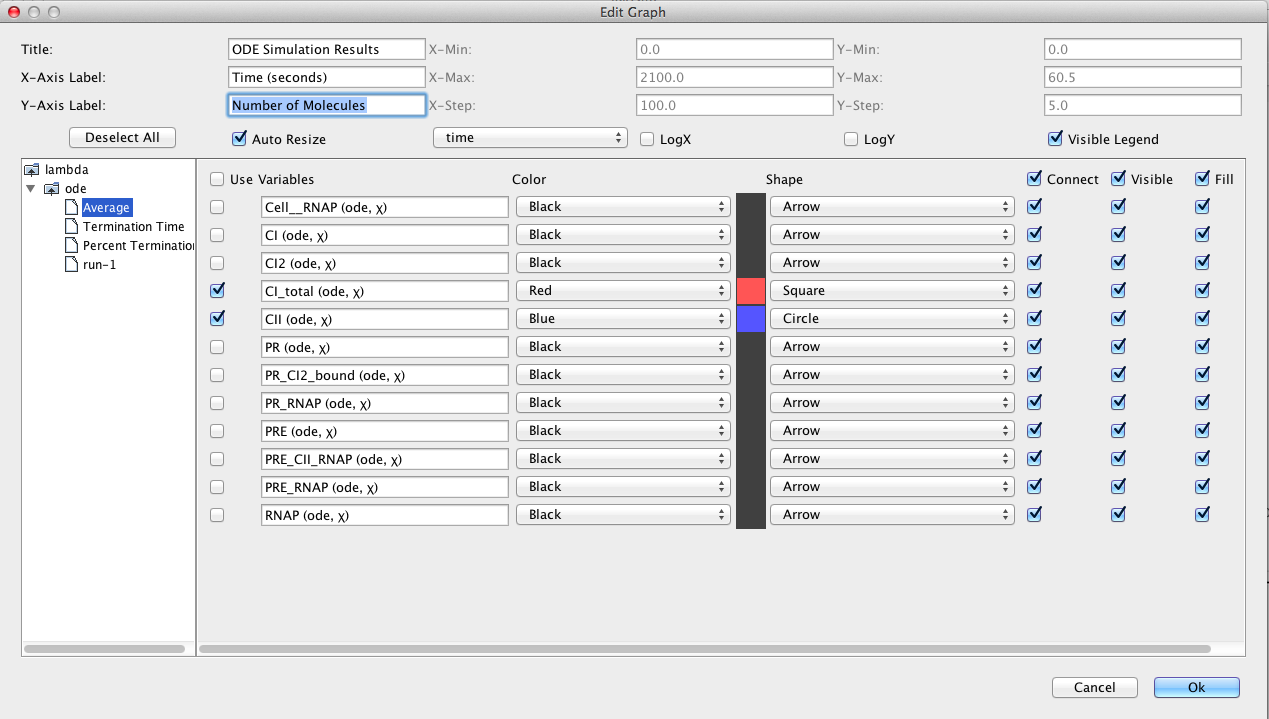
\includegraphics[width=160mm]{screenshots/odeResults}\\
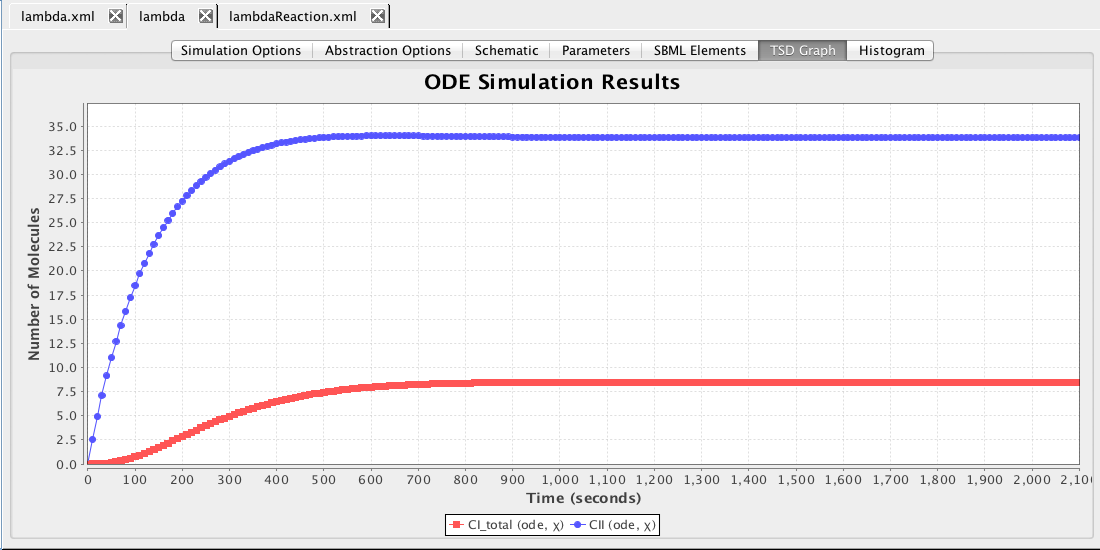
\includegraphics[width=160mm]{screenshots/odeSimResults}
\end{center}

Graphs can be exported in a variety of formats including:
\begin{itemize}
\item Time series data format (tsd).
\item Comma separated value (csv).
\item Column separated data (dat).
\item Encapsulated postscript (eps). 
\item Joint Photographic Experts Group (jpg). 
\item Portable document format (pdf).
\item Portable network graphics (png). 
\item Scalable vector graphics (svg).
\end{itemize}
In order to export a graph, you can either click on the Export icon 
\includegraphics{../gui/icons/export} or select one of the graph export options from the File menu.  When using the Export icon, the type of file exported will depend on the extension provided to the file name.  Click on the Export icon, browse to a location on your file system, and enter the file name of {\tt ode.pdf} to create a PDF file for your graph.

\begin{center}
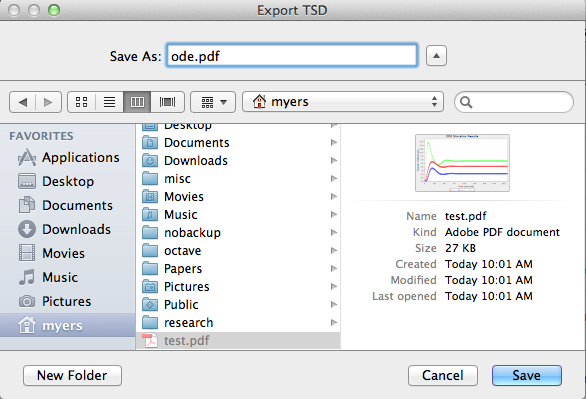
\includegraphics[height=60mm]{screenshots/exportTSD}
\end{center}

Now, select the Simulation Options tab again, select {\tt Monte Carlo}, change the number of runs to 100, set the simulation ID to {\tt ssa}, and click on the Save and Run icon.  Click on the TSD Graph tab.  Double-click on the graph to bring up the graph editor.  Open the {\tt ssa} simulation directory, and highlight {\tt run-1}.  Select CI\_Total and CII, change the title to ``SSA Simulation Results'', change the X-Axis Label to ``Time (seconds)'', and change the Y-Axis Label to ``Number of Molecules''.  Press the OK button.  Click on the Export icon and enter the file name {\tt ssa-1.pdf}.  Repeat these steps to generate graphs for the average ({\tt average.pdf}) and standard deviation ({\tt stddev.pdf}).  Note that you can use the ``Deselect All'' button to remove all items from the graph.

\begin{center}
\includegraphics[width=160mm]{screenshots/ssaSim}\\
\includegraphics[width=160mm]{screenshots/ssaResults}\\
\includegraphics[width=160mm]{screenshots/ssaSimResults}
\end{center}

Another way to view simulation results is on the schematic.  To do this, click on the schematic tab.  At the bottom of the window, select the Choose Simulation button, which brings up a window with all the simulations in this analysis view.  Open the {\tt ssa} directory, select {\tt run-1.tsd}, and press OK. 

\begin{center}
\includegraphics[width=160mm]{screenshots/chooseSim}
\end{center}

Now, click on the CI species, which brings up the Edit Species window.  Select the Appearance tab.  Here you can select how you want the species to appear as you playback the simulation.  You can have it change color, size, and/or opacity on a gradient.  You can also select the range of molecule counts to specify the ends of the gradient(s).  Finally, you can indicate that these selections are either for this species or all species in the model.  For our example, let's make CI follow a green color gradient, CI2 follow a red color gradient, and CII follow a blue color gradient.
\begin{center}
\includegraphics[width=160mm]{screenshots/editSpeciesAppearance}
\end{center}

Once you have made your selections, you can now play back the simulation.  You can either single-step the simulation by pressing the \includegraphics{../gui/icons/modelview/movie/single_step} icon or play continuously by pressing the \includegraphics{../gui/icons/modelview/movie/play} icon.  The playback can also be paused by pressing the \includegraphics{../gui/icons/modelview/movie/pause} icon and restarted by pressing the  \includegraphics{../gui/icons/modelview/movie/rewind} icon. 

\begin{center}
\includegraphics[width=160mm]{screenshots/movieView}
\end{center}

Using the schematic tab, you can also adjust initial values and parameters allowing one to perform simulations to determine the effect of these changes.  Clicking on any species, promoter, reaction, or influence brings up the corresponding editor.  To change a value, switch the corresponding combo box to modified, which will then allow you to change the value.  For example, as shown below, we have reduced the degradation rate for CI to 0.00075.  Now, rerun the simulation and observe the change in the simulation data.

\begin{center}
\includegraphics[width=160mm]{screenshots/paramEdit}
\end{center}

In addition to making single changes, you can also sweep a value as shown below.   When you click on the Sweep button, it brings up a window where you can select the start value, the stop value, and the step value.  Using the values shown below for this example, simulations are generated using degradation rates of 0.001, 0.003, 0.005, and 0.007.  The level indicates how the sweep should perform when multiple variables are swept at the same time.  Variables at the same level are changed at the same time.  Furthermore, all variables on level 2 are stepped through all their values before changing the values of those variables on level 1.  After the values on level 1 are changed, the values on level 2 are stepped through all their values again.  Rerun the simulation and create a graph that shows the value of CI for each of the different degradation rates.

\begin{center}
\includegraphics[width=160mm]{screenshots/sweep}
%\includegraphics[height=90mm]{screenshots/sweepPR}
\end{center}

The efficiency of simulation can be improved by employing various automatic abstraction techniques.  Go back to the Schematic tab and change the degradation rate of CI back to the default value.  Also, go to the SBML elements tab and uncheck the rule for CI\_total.  To activate abstraction, click on the Simulation Options tab, select Abstraction and change the simulation ID to {\tt abs}.  Press the Save and Run icon and note that the simulation time is substantially faster.  Plot both the SSA results for CI\_total and CII with the abstraction results for CI (note this is now equivalent to CI\_total after abstraction) and CII.

\begin{center}
\includegraphics[width=160mm]{screenshots/absResults}
\end{center}

One way to understand why abstraction is so much faster is by looking at the complexity of the reaction-based model before and after abstraction.  The reaction-based model after abstraction is shown below which is clearly much simpler than the full model shown earlier.

\begin{center}
\includegraphics[width=100mm]{screenshots/viewNetworkAbs}
\end{center}

Next, let's try checking some properties.  To do this, go to the SBML Elements tab and check the boxes next to the constraints.  Recall that these constraints terminate simulation whenever CI goes above 20 molecules or CII goes above 50 molecules.  Go back to the Simulation Options tab and change abstraction back to none, the Simulation Type to Monte Carlo, and Simulation ID to prob, then press the Save and Run icon.  Now, let's plot the results on a histogram by clicking on the Histogram tab and then double-clicking on the graph to bring up the histogram graph editor shown below.  Open the prob folder, select the sim-rep file, and check the Use check box to get all fields.  

\begin{center}
\includegraphics[width=160mm]{screenshots/editProbGraph}
\end{center}

The histogram shown here indicates that CI goes above 20 molecules first about 21 percent of the time, CII goes above 50 molecules first about 74 percent of the time, and the simulation terminates before either happens about 5 percent of the time.

\begin{center} 
\includegraphics[width=160mm]{screenshots/probResults}
\end{center}

These results can also be visualized using the TSD graph tool.  Click on the TSD graph tab, click on the graph, Deselect All, open the prob folder, select the Percent Termination file, and add both constraints to the graph.  The result, shown below is the probability of each constraint terminating the simulation as time evolves.  

\begin{center} 
\includegraphics[width=160mm]{screenshots/probResultsTSD}
\end{center}

\section{Learn Tool}

This section describes how a model can be learned from time series data using {\tt iBioSim}'s Learn Tool.  To demonstrate the Learn Tool, first create a simple model, {\tt lambdaLearn}, which just includes the two species CI and CII as shown below.  Next, create a learn view by right-clicking on this model file and selecting Create Learn View.  Give this learn view the ID {\tt learnLambda}.  At this point, a new learn view should open.  You should also notice that an icon appears next to your model file.  When you click on this, it will show you all of the analysis and learn views associated with this model.

\begin{center}
\includegraphics[height=60mm]{screenshots/createLearn}
\end{center}

The next step is to add some experimental data from which you wish to learn a model.  In this demo, we will just utilize our simulation data as synthetic experimental data.  To do this, click Copy From View, and select {\tt lambda/abs}.  Highlight {\tt lambda/abs/run-1.tsd} and you should see the simulation data for CI and CII appear on the right in the data editor. 

\begin{center}
\includegraphics[width=160mm]{screenshots/dataManager}
\end{center}

Now, click on the Learn tab.  Here you can edit the various learning options.  For example, you can either use auto-generated levels or user-generated levels for your data encoding.  Select Use User Generated Levels, which will make the levels below editable.  At this point, you can ask the tool to suggest levels by clicking on the Suggest Levels button.  Finally, click on the Save and Run icon which will bring up the model that has been learned from this experimental data using Graphviz's dotty program, and ask you for a model ID for the generated model.  

\begin{center}
\includegraphics[width=160mm]{screenshots/learn}
\end{center}

\section{Advanced Modeling}

This section is less detailed than the others but it gives some intuition about modeling using reactions, components, and grids.  

%% TODO: Need to add SBOL to tutorial

%It also introduces our preliminary support of the emerging \emph{Synthetic Biology Open Language standard} (SBOL).  Let us take the last of these first.  An SBOL file includes \emph{Collections} of \emph{DNA Components}.  Each DNA component has a unique ID, name, description, type, and a DNA sequence.  A DNA component can be a simple sequence feature like a promoter, ribosome binding site, open reading frame (i.e., gene), or terminator.  It can also be an annotated DNA sequence that includes several of these individual features, perhaps organized hierarchically.  For example, a DNA component may include a promoter followed by a ribosome binding site followed by a open reading frame followed by a terminator.  When editing the model, you may have noticed the various SBOL fields.  Namely, for a promoter, you can associate both a DNA component to the promoter as well as a terminator for the transcription initiated at this promoter.  For a species, you can associate both a DNA component for the open reading frame for the gene that produces this species as well as the ribosome binding site where translation begins for this gene.  This SBOL browser is opened by clicking on an Associate SBOL button within either the Species Editor or Promoter Editor.  This browser only shows DNA components of the appropriate type.  For example, when associating a species to its open reading frame, only DNA components of the open reading frame type are shown.  After you have associated all genetically produced species (i.e., CI and CII in our model) and all promoters (i.e., PR and PRE in our model), you can then save the DNA component for your model into your SBOL file.  You can also export it into a new or existing SBOL file outside your project.
%
% \begin{center}
% \includegraphics[width=160mm]{screenshots/AssociateSBOL}
% \end{center}
%
First, let's consider an alternative model of CII degradation which we are going to model using chemical reactions.  To do this, create a new model named {\tt CII\_degradation}.  In this model, create species CII, P1, and CII\_P1, making CII have the input type so that we can connect to it later.  Set an initial amount of 35 molecules for P1.

\begin{center}
\includegraphics[width=160mm]{screenshots/P1}
\end{center}

Now, select the Add Reaction icon \includegraphics{../gui/icons/modelview/add_reaction_selected} and click on the schematic canvas to drop a reaction.  This creates a reaction with a default ID and parameter values that we can change later, if we wish.

\begin{center}
\includegraphics[width=160mm]{screenshots/reaction}
\end{center}

Now, let's connect up the reactant species.  To do this, select the Reaction icon \includegraphics{../gui/icons/modelview/reaction_selected}, select the reactant species CII, and, while holding the mouse button, drag the reaction edge to the reaction R1.  Similarly, add P1 as a reactant as well.  If you double-click on a reactant edge, it brings up a Reactant editor where you can change the stoichiometry, if desired.

\begin{center}
\includegraphics[width=160mm]{screenshots/reactant}
\end{center}

Connecting product species is accomplished in much the same way, except in this case you select reaction R1 and drag the reaction edge to the product CII\_P1.  Again, there is a Product editor for changing the stoichiometry.  Note that modifiers (i.e., species that are neither produced nor consumed by a reaction but simply catalyze a reaction) can be added in a similar way using the Modifier icon \includegraphics{../gui/icons/modelview/modifier_selected} instead.

\begin{center}
\includegraphics[width=160mm]{screenshots/product}
\end{center}

Now, let's adjust the parameters for this reaction by clicking on it to open the Reaction Editor. Press the Use Mass Action button to automatically create a kinetic law for this reaction.  Then, make this reaction reversible and adjust its forward reaction rate to be 1.0.  

\begin{center}
\includegraphics[width=160mm]{screenshots/localParam}
\end{center}

Follow the same steps to add another reaction that degrades CII in the CII\_P1 form and releases the protease molecule P1.  This reaction is not reversible and it should have a forward rate of 0.002.

\begin{center}
\includegraphics[width=160mm]{screenshots/kineticLaw}
\end{center}

Let's now go and add this new degradation mechanism to our lambda model (you might actually want to copy your old model before you do this, which you can do by highlighting the file and selecting Edit $\rightarrow$ Copy or using the right mouse button menu).   To simplify things, remove the rule, constraints, and event.  Next, open the Species Editor on CII and deselect the degrades option.  Finally, select the Add Component icon \includegraphics{../gui/icons/modelview/add_component_selected} and click on the Schematic canvas opening the Add Component(s) window.  In this window, browse the combo box to find your CII\_degradation model.  Pressing OK will then add it to your schematic.

\begin{center}
\includegraphics[width=160mm]{screenshots/addComponent}
\end{center}

Now, let's connect CII to this new component to relate the CII within the component to the outer CII species.  To do this, select the CII species and, while holding the mouse button, drag a connection to the component connecting CII to the CII port on the component.  
You may want to now go and try simulating this model, if you like.

\begin{center}
\includegraphics[width=160mm]{screenshots/addPort}
\end{center}

In the last example, we will build a model with a grid. First, edit the CII species and make it diffusible, and save the model.  Now, create a grid model using the File $\rightarrow$ New $\rightarrow$ Grid Model menu, and name the new model {\tt Population}.  In the create grid window shown below, select your copy of your lambda model and change the number of rows and columns to 5.  

\begin{center}
\includegraphics[width=60mm]{screenshots/createGrid}
\end{center}

The schematic in a grid model is a bit different.  It includes a grid in which each location can be empty or contain exactly one component.  Only components can be added to grids.

\begin{center}
\includegraphics[width=160mm]{screenshots/gridModel}
\end{center}

When you create a reaction-based model for a grid during analysis, reactions are created to move the diffusible species between the grid locations to provide a coarse form of spatial modeling.  If the component within a grid location is enclosed in a compartment membrane (indicated by the rounded corners), the model generated also includes reactions to diffuse the species in and out of the compartment.  In the analysis schematic, you can visualize your grid models by clicking on the component in the grid and selecting the species that you would like to see.  For each such species, you can set its color, size, and/or opacity gradient.  You can also copy these settings to all like models in your grid.  Finally, you can click on the area outside of the component within the grid to allow you to also visualize the species that are in the medium.

\begin{center}
\includegraphics[width=160mm]{screenshots/compAppearances}
\end{center}

%% TODO: Add Petri net modeling

\noindent
A more detailed 
%%tth:\begin{html}<a href="iBioSim_Grid_Tutorial.html">\end{html}
grid tutorial
%%tth:\begin{html}</a>\end{html}
is available in the {\tt docs} directory that comes with the distribution.

\end{document} 
